\chapter{Methodology}
\label{chapter:method}

An information system architecture that supports care planning of pressure ulcers requires certain basic functionalities such as 
\begin{itemize}
	\item capturing bio-mechanical data of the body
	\item Analyzing those data
	\item collecting risk assessment data
	\item providing platform to report and document ulcers
	\item networking related people
	\item planning schedules.
\end{itemize}

Therefore our information system architecture is supported by pressure sensing mats and mobile apps. Some standard risk assessment scales, ulcer documentation formats are added to the system with appropriate modifications. Additionally scalability, flexibility and cost-effectiveness are two other important characteristics of such system. Our initial scope was to build a pressure sensing mattress system that is capable of recommending optimal repositioning strategies based on bio-mechanical data. As there are no proper evaluation criteria to assess pressure ulcer  prevention and the existing bio-mechanical and pathological research in pressure ulcers are inconclusive, we constructed an information system that provide a platform to investigate pressure ulceration phenomenon while providing a tool for care planning by digitizing processes currently done in paper or not done in any systematic way. Existing theories can be used in our system to improve care planning within their limitation.

\section{Components and Functionality}

There are three main components of our solution. 
\begin{itemize}
	\item Information System (Server and Backend)
	\item Mobile App
	\item Pressure sensing matress
\end{itemize}

\begin{figure*}[t]
    \vspace{-0.7cm}
      \centering
      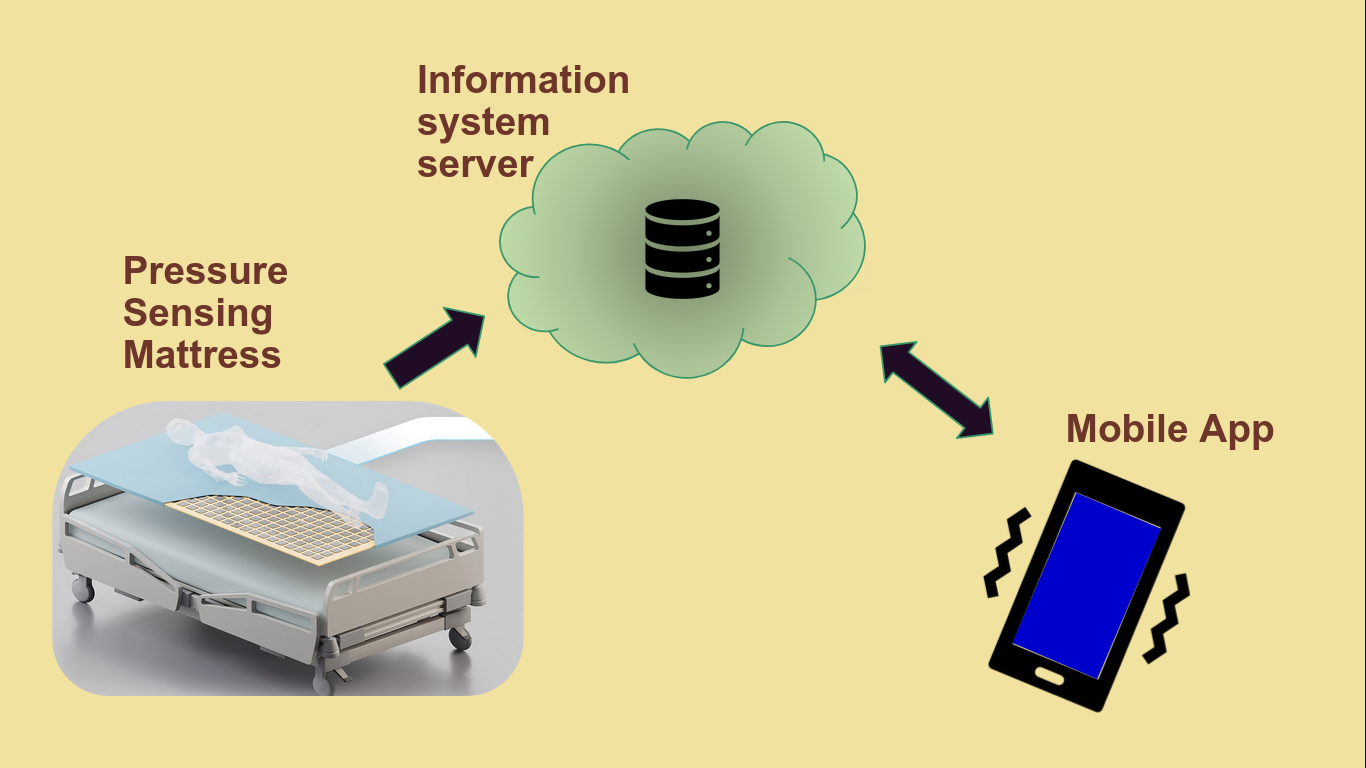
\includegraphics[width=0.5\textwidth]{figs/component-diagram.png}
      \vspace{-0.2cm}
      \caption[Component Diagram]{Component diagram}
      \label{fig:components}
\vspace{1.0cm}
\end{figure*}
The information system provides basic components of authentication, and data storage for pressure data, personal risk assessment data and ulcer documentation. It is consist of another supplementary subcomponent for machine learning models. The information system provides a RESTful API for mobile app clients and pressure sensing mats. App and pressure sensing mat can send and retrieve relavent information from the information system. The mobile app provides user interface for patients/guardians, caretakers and doctors to interacts with the system.

The pressure mat consist of a sensor panel developed by a substrate of piezo-resistive material Velostat\textsuperscript{\textregistered}. The sensor readings are processed one cell by one in the ATMega32\textsuperscript{\textregistered} microcontroller and send to the information system using a NodeMCU/ESP8266\textsuperscript{\textregistered} via Wifi and internet. The information system is capable of integrating other available commercial pressure sensing mattresses without any change of its structure.

In the central server of the information system these pressure data will be filtered and stored. The sleeping postures and ulceration points are identified by these data and pressure at these points is saved in a seperate table using Neural Network Models.

There is a notificaation system that sends notifications to the caretakers of patients instructing the repostitioning plan.
\begin{figure*}[t]
    \vspace{-0.7cm}
      \centering
      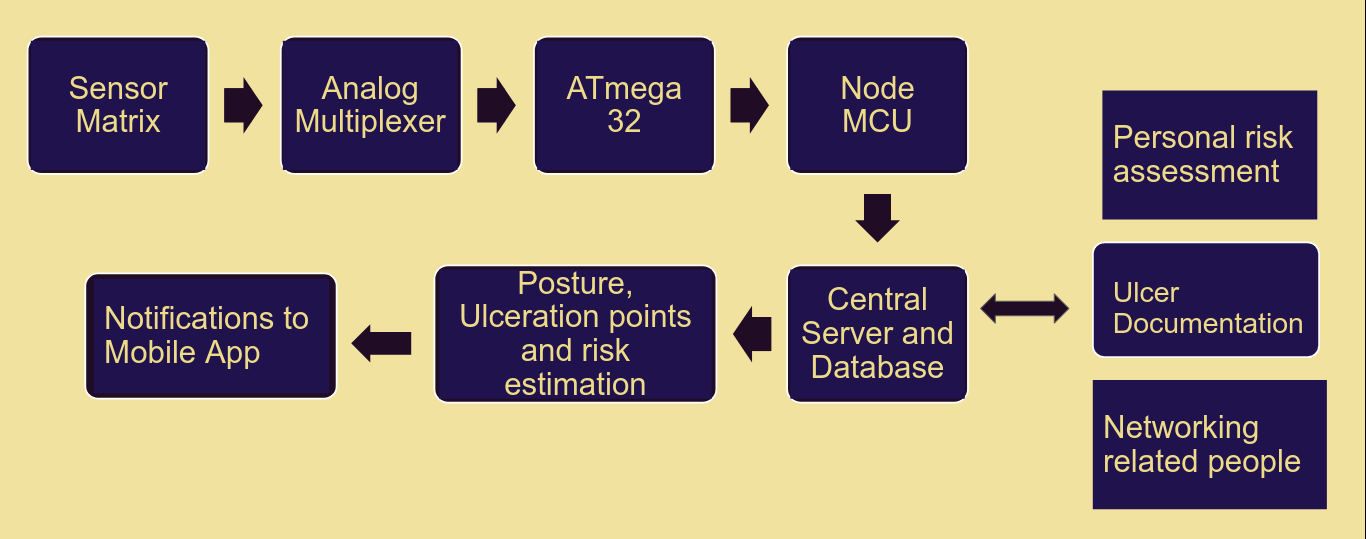
\includegraphics[width=0.9\textwidth]{figs/functional_block.png}
      \vspace{-0.2cm}
      \caption[Functional Block Diagram]{Functional block diagram}
      \label{fig:functional}
\vspace{1.0cm}
\end{figure*}

\section{Information system back-end}

Information system backend is written in Python using the enterprise level web fullstack designing framework Django\textsuperscript{\textregistered} and hosted in Heroku\textsuperscript{\textregistered} cloud platform. As the database management system we choose Postgresql which is a SQL based relational database management system. All the static media files are stored in a Cloudinary S3 bucket\textsuperscript{\textregistered}. APIs are created from django-rest-framework library and Firebase\textsuperscript{\textregistered} is used to communicate with mobile apps with push notifications. 

The web application considered on Django apps (submodules) for each main functionality.
\begin{enumerate}
	\item Authentication and User Profiles
	\item Social connection handling
	\item Pressure data
	\item Personal Risk Analysis
	\item Ulcer Documentaion
\end{enumerate}

Neural network models are build and trained using Tensorlfow\textsuperscript{\textregistered} and Keras\textsuperscript{\textregistered} libraries and hosted in Heroku\textsuperscript{\textregistered} using popular python backend microframework Flask\textsuperscript{\textregistered}.


\subsection{Authentication and Authorization}

There are user accounts to authenticate the users and there are three groups as doctors, caretakers and patients. These roles and accounts are used to authorize access to particular components. Only users have write or update permission to their personal information, care takers can update there risk assessment data while doctors can update ulcer reporting documentation as well as risk assessment data. Even latter data only accessible to caretakers or doctors who are assigned to relevant patients. Token authentication is used to authenticate access.

To create and account a user is requested to add his username and password and there after he has to use that username and password to log in. Users can update their profile with basic details and profile photos.

\subsection{Social Networking}

All doctors, caretakers, patients can be see each other in search lists. The connection between the users are established via request and confirm mechanism. There are send, show, accept, reject, delete functionalities for a request. Doctors and caretakers can only access data of a patient only if they has been connected to the particular patient. Users can remove others from there connection list. 

\subsection{Pressure data}

Pressure data sent from pressure mats are stored in the database via the central server. These data are further analysed with Neural Network Models to find ulceration points. Pressure data is stored in the format \textbf{lx, ly, x, y, p, n} format. 

Here,

\begin{description}
	\item[lx]: Number of cells over x axis of the mat 
	\item[ly]: Number of cells over y axis of the mat 
	\item[x]: x coordinate of the current cell 
	\item[y]: y coordinate of the current cell  
	\item[p]: Pressure at the (x,y) cell
	\item[n]: frame number (Reading complete mat is a one frame)  
\end{description}

This format supports to send cells one by one therefore we can capture even a partial reading. This format do not restrict the resolution to a particular value we decide so changing lx and ly of the request any available pressure sensing mattress can be integrated without any structural change of the system. 

\subsection{Machine Learning}

There are two machine learning models to analyze pressure data. One is to identify posture and the other is to identify ulceration points. Since the ulceration occurs in these particular sites it is important to identify pressure at those locations. To locate this points on the pressure mat and to identify repositioning we should find postures of the patient from pressure data. 
We used a dataset by university of Dallas to train the neural networks and we used data preprocessing and augmentations to improve the model. There are 13 people in 18 postures (5 major postures supine, left yearning, right yerning, left fetal, right fetal and there slight varaiations with rolling angle and using pillows as wedges.) There are collection of pressure distribution measured by a commercial pressure measuring mattress for 2 mins which is roughly 120 frames for each. The resoulution is 64 $\times$ 32.

\subsubsection{Posture Detection Model}

Posture detection model is a sequential model with several convolution and pooling layers before final dense layers. When the input pressure image is given the model outputs the corresponding name of the sleeping posture.
\begin{figure*}[t]
    \vspace{-0.7cm}
      \centering
      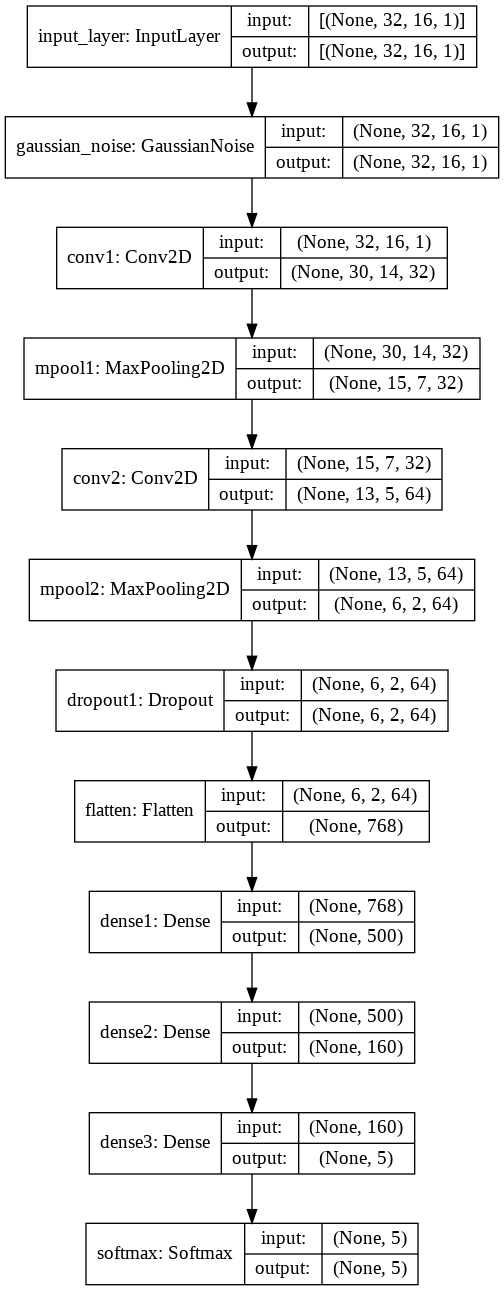
\includegraphics[width=0.3\textwidth]{figs/posturemodel.png}
      \vspace{-0.2cm}
      \caption[Posture Detection Model]{Neural Network architecture of the posture detection model. When pressure image is given the model identifies the sleeping posture}
      \label{fig:posturemodel}
\vspace{1.0cm}
\end{figure*}

\begin{description}
	\item[Validation] The dataset was divided into a training and holdoutset such that data from 9 persons for train and data from 4 persons for holdout.
	\item[preprocessing] The pressure images are resized to 32 $\times$ 16, Gaussian noise of variation of 0.08 is added and finally Gaussian filter of variation of 0.5 is applied. This adding extra noise is supposed to regularize the neural network to work in more realistic environments with low cost pressure mattresses.
	\item[Data Augmentation]  Pressure images are rotates in random angles between by -150 to -150 and Gaussian Noise of variance of 0.1 is added.	
\end{description}

The 5 labels for supine, left yearning, right yerning, left fetal and right fetal are onehot encoded. 

Neural network provided 92.45\% holdout set accuracy.


\subsubsection{Ulceration Point Detection Model}

The same datset was used to train the neural network model for ulceration point detection. We manually created bounding boxes for ulceration points using the annotator tool Labelbox\textsuperscript{\textregistered}. Then we preprocessed images likewise in the previous model. \begin{figure*}[t]
    \vspace{-0.7cm}
      \centering
      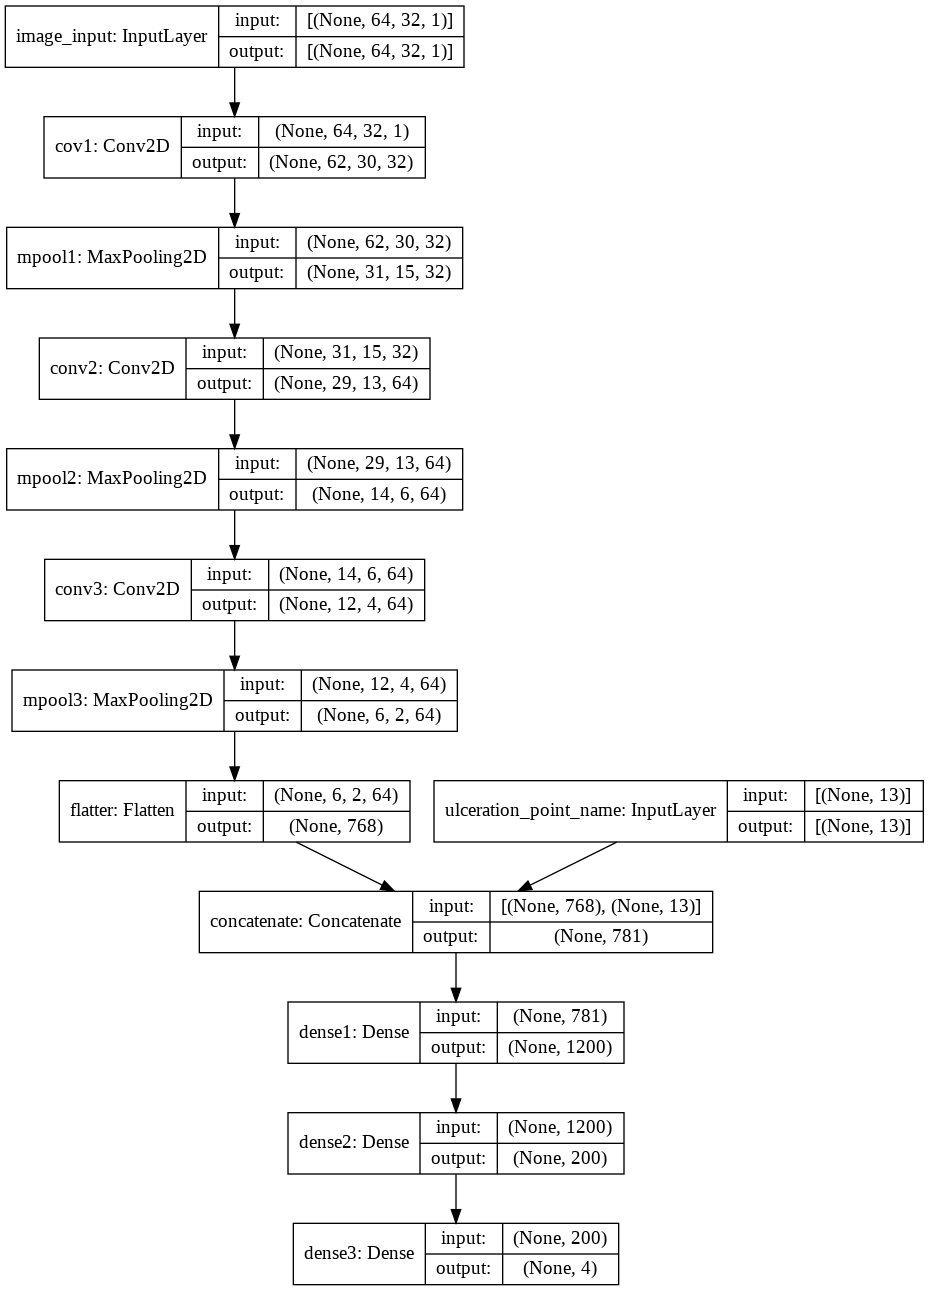
\includegraphics[width=0.6\textwidth]{figs/ulceration_point.png}
      \vspace{-0.2cm}
      \caption[Ulceration point model]{Neural Network architecture of the model for ulceration point detection. When the pressure image and the ulceration points we consider is  given the model provides parameter of the bounding box for that particular site.}
      \label{fig:posture_model}
\vspace{1.0cm}
\end{figure*} The four paramters (two coordinates of the upper left corner of the bounding box, height and width) were used to train the model with a mean squared error loss function. There are two inputs to the model. The pressure image and the name of the ulceration point we consider (onehot encoded). Then the model outputs four parameters for the bounding box. 


\subsection{Scheduling}

Usually 2h recommendation period for any posture is used an there is no particular order of posture order. However the researchers of University of Dallas tried to find a repostition schedule based on pressure distribution. Unfortunately there risk assessment metric is based on data from closely related research for slightly different problems and their final result is depend on ad-hoc assumptions they used. 

In summary if we put the outline of their research perspectively it states that the supine posture is more risky as the both sides of the body is subjected to pressure. Although a side of body subjected to more pressure in left or right posture that is a complete relieving phase for the other side of the body. Although we hessitate about the validity of their arbitrary risk metric and ad-hoc assumption we decided to use their result and recommend a repositioning plan as follows. \begin{figure*}[t]
    \vspace{-0.7cm}
      \centering
      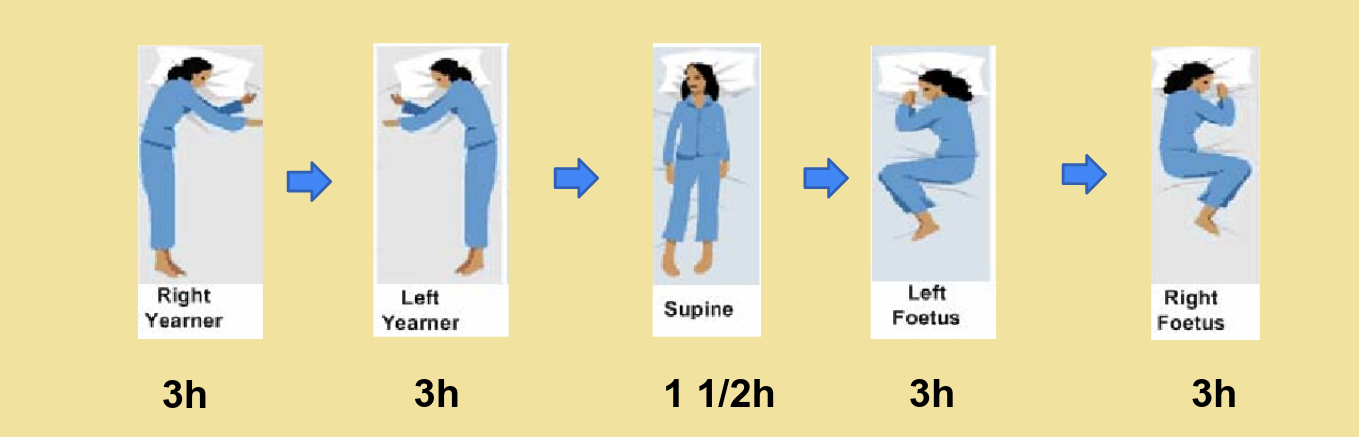
\includegraphics[width=\textwidth]{figs/schedule.png}
      \vspace{-0.2cm}
      \caption[Repositioning Schedule]{Schedule for reposition.}
      \label{fig:schedule}
\vspace{1.0cm}
\end{figure*}

\begin{enumerate}
	\item Right Yearning - 3 h
	\item Left Yearning - 3 h
	\item Supine - 1.5 h
	\item Left Fetal - 3 h
	\item Right Fetal - 3 h
\end{enumerate}

The left and right postures should be alternatively applied but we do not distinguish between yearning and fetal. As this intervals are below the range of NICE guidelines it could be justified to use these intervals. 

\subsection{Personal Risk Assessment}

We considered two existing personal risk assessment scales Braden scale and Waterloo scale. The information system captures data relevent to both scales and calculate corresponding metrics. 

The personal risk assessment forms contains following data and expected to be filled by a health care professional (a doctor or a nurse). 

\begin{description}
	\item[Assessed By]: The doctor or the caretaker (nurse) assessed personal risk
	\item[Gender]: Male/Female
	\item[Age]: Age of the patient
	\item[Weight]: Weight of the patient (kg)
	\item[Height]: Height of the patinet (cm)    
\end{description}

These details should be filled as 1,2,3,4 according to the Braden scale guideline. 

\begin{description}
	\item[Sensory perception]: Ability to respond meaningfully to pressure-related discomfort 
	\item[Moisture]: Degree to which skin is exposed to moisture 
	\item[Activity]: Degree of physical	activity 
	\item[Mobility]: Ability to change and control body position
	\item[Nutrition]: Usual food intake 	pattern 
	\item[Friction and Shear]     
\end{description}

Explicit definition of 1,2,3,4 levels for each category is given in the Braden scale guideline (which is showed by an information box in the mobile app.)

According to the total score the patients are classified into four risk categories.


\begin{tabular}{l r}
	Severe risk &  $\leq$ 9\\
	High risk &  10 - 12\\
	Moderate risk & 13 - 14\\
	Mild risk &  15 - 18 \\
\end{tabular}\\

These are some other important risk factors (Yes/No binary options). 

\begin{itemize}
	\item Diabetes mellitus
	\item Peripheral vascular disease
	\item Cerebral vascular accident
	\item Hypotension
	\item Hypoalbuminemia
	\item Incontinence
	\item Venus thrombosis	
\end{itemize}


\subsection{Ulcer documentation}

Documenting existing ulcers is an important concern. Treatments are based on proper documentation. This includes basic details related to the wound, surrounding skin and conditions of the patient. We adopted basic components from NPUAP (National Pressure Ulcer Advisory Panel) guidelines and SOS (State of Oklahoma) toolkit to prepare our documentation patteren. We discussed the current state of pressure ulcer documentation with a medical practitioner in Sri Lanka and remove overcomplicating components from these two guidelines. Then we add several additional components and alter the terminology in order to make compatible with medical terminology used in Sri Lanka. Some of the components we introduce here are not currently documented in Sri Lanka. 

\begin{description}	
	\item[Reported by]: The doctor that reports the ulcer
	\item[ChangeAddDelete]: The updated date (automatically filled)
	\item[Site]: Ulceration points
	\item[Stage]: Stage I,II,III,IV, DTI (Deep Tissue Injury), Unstaged  (NPUAP classification)
	\item[Duration]: Duration (days)
	\item[Length]: Length of the ulcer (mm)
	\item[Width]: Width of the ulcer (mm)
	\item[Depth]: Depth of the ulcer (mm)
	\item[Margin]: Regular, Irregular 
	\item[Edge]: Sloping, Punched out, Rollout, Everted
	\item[Edge color]: Color of the edge of the ulcer
	\item[Underminings]: (Yes/No)
	\item[Sinus tracts]: (Yes/No)
	\item[Floor]: Healthy, Granualation Tissue, Slough, Necrotic, Eschar, Epithelial (Multiple selection)
	\item[Discharge]: Serous, Purulent, Serosanguineous, Other  
	\item[Discharge amount]: Small, Medium, Heavy 
	\item[Surrounding skin]: Warm, Thickend, Hyperpigmented, Hypopignmented, Gangreous, Itching, Swelling (Multiple selection)
	\item[Skin sensation]: Good, Impaired    
	\item[Regional lymph nodes enlarged]: Yes/No
	\item[Smell]: Yes/No
	\item[Pain]: Yes/No
	\item[Progress]: Improved, No change, Stable, Decline
	\item[Image]: Image of the ulcer
\end{description}




\section{Mobile app} 

Mobile app provides a user interface for basic funcionalities of the system. This includes,
\begin{itemize}
	\item Login
	\item Profile update
	\item Search other users
	\item Handle social connections
	\item Register mattress
	\item Personal Risk Assessment
	\item Ulcer documentation
	\item Notification
\end{itemize}

Notifications are  send 5  mins prior to the reposition and another at the moment reposition is planned. Next posture and the period in that posture is given with the notification. If the patient is not turned at the specified time then another notifications are send three times with a 5 min interval.


\section{Pressure Mat}

There are two difference methods to create a pressure mat. The first method is to combine large number of sensors and the second method is to devevlop a single substrate of pressure sensing material into a sensor panel. First approach is manufacturably complex. Therefore we selected second approach. Velostat\textsuperscript{\textregistered} is a low cost piezo-resistive material that is used for similiar applications. Selection of piezoresistive material over piezocapacitive material reduce complexity of the senosor interfacing. Resistance can be measured constructing a voltage divider. 

\subsection{Calibration of the Material}

\begin{figure*}
    \vspace{-0.7cm}
      \centering
      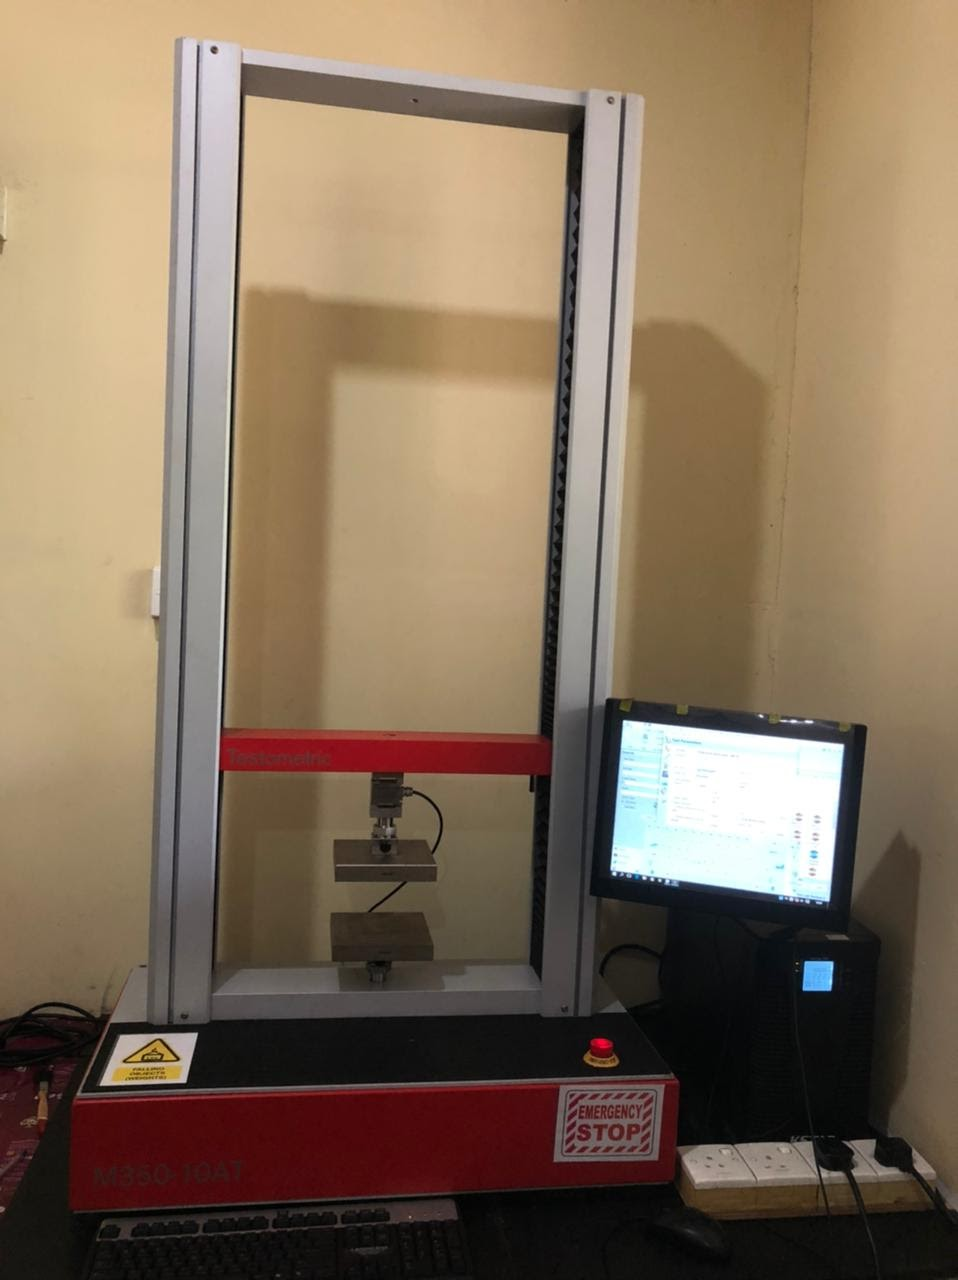
\includegraphics[width=0.5\textwidth]{figs/utm.jpg}
      \vspace{-0.2cm}
      \caption[Universal Testing Machine]{Universal testing machine}
      \label{fig:utm}
\vspace{1.0cm}
\end{figure*}
\begin{figure*}
    \vspace{-0.7cm}
      \centering
      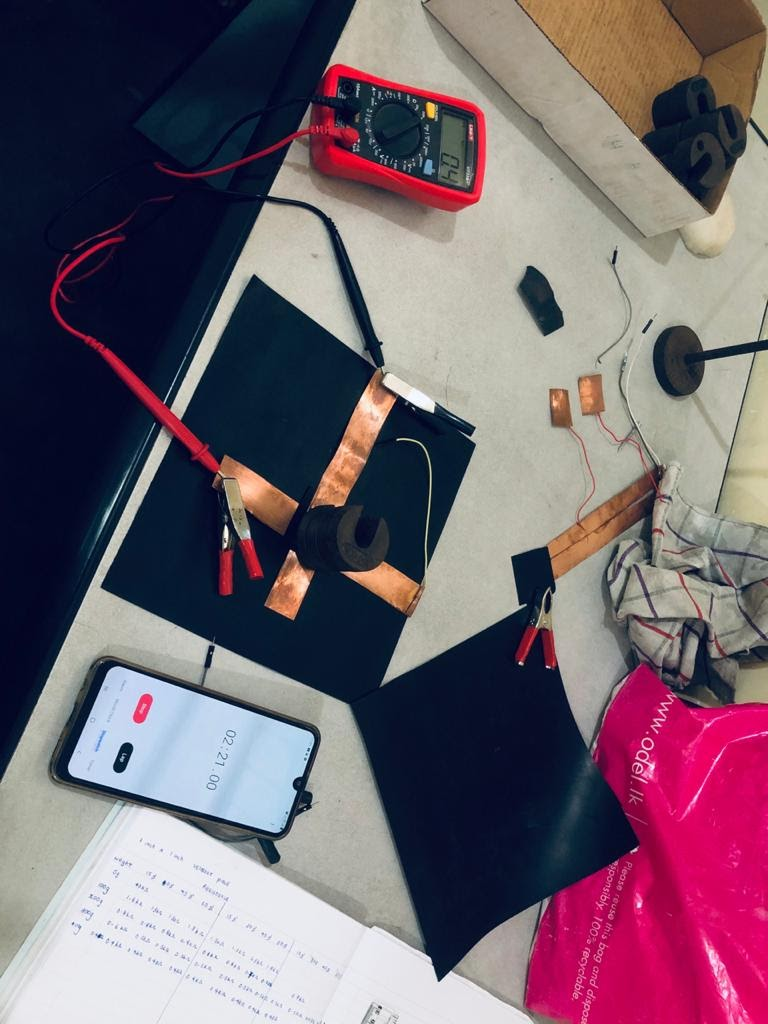
\includegraphics[width=0.5\textwidth]{figs/deadweight.jpg}
      \vspace{-0.2cm}
      \caption[Measuring with Deadweight]{Measuring with deadweight}
      \label{fig:deadweight}
\vspace{1.0cm}
\end{figure*}


\subsection{Preparing Mat}

Velostat sheet was sandwiched by two Neoprene sheets each one contains set of parallel rows or columns of copper tapes. Each column is attached to the output channels of an analog multiplexer and each rows are attached to the input channels of two multiplexers that works as a one multiplexer in combine. 

\begin{figure*}
    \vspace{-0.7cm}
      \centering
      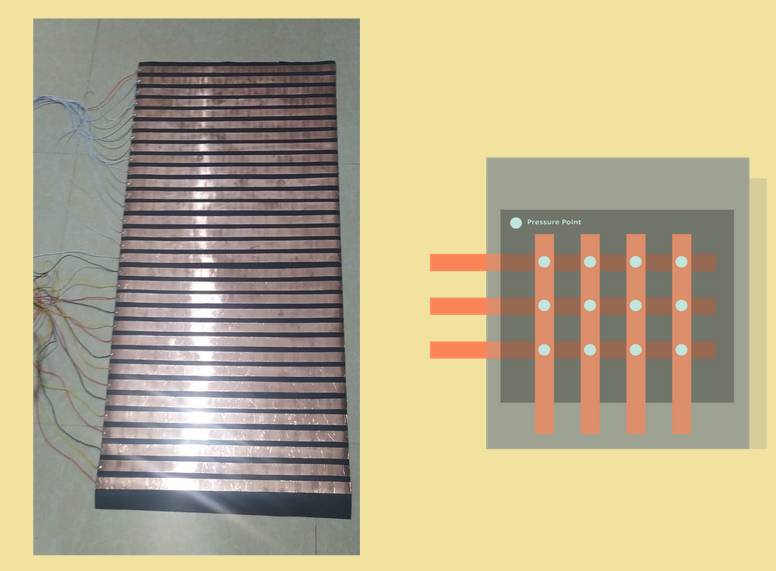
\includegraphics[width=0.5\textwidth]{figs/pressure_mat.png}
      \vspace{-0.2cm}
      \caption[pressuremat]{Pressure mat}
      \label{fig:pressuremat}
\vspace{1.0cm}
\end{figure*}

Columns are powered one by one using the analog multiplexer and the voltage is measured over a voltage divider choosing each row by other multiplexers. 

Neoprene acts as an insulator to build the copper wire grid. All rows are weakly pulled down according to previous research which shows it reduce cross-talk effects.

\subsection{Sensor reading processing and communication}
The communication between ATMega32 and ESP8266 is via UART and then the WIFI server sends it to server. 






